%Correct the file name.
%X: book number
%Y: part number
%ZZZ: page number in three digits. So page 3 would be 003.



\documentclass[11pt]{amsbook}

\usepackage{../HBSuerDemir}	% ------------------------
\usepackage{eufrak}
\usepackage{amsmath}
\usepackage{mathtools}
\usepackage{dsfont}
\DeclarePairedDelimiter{\abs}{\lvert}{\rvert}
\begin{document}

% ++++++++++++++++++++++++++++++++++++++
\hPage{feyzioglu-101}
% ++++++++++++++++++++++++++++++++++++++
\textbf{Proof:} We must find a one-to-one correspondence between $\mathfrak{R}$ and $\mathfrak{L}$.
We put: \hspace{7em}$\sigma :\mathfrak{R} \rightarrow \mathfrak{L}$

\hspace{8em} $H a \rightarrow a^{-1} H$ 

We show that $\sigma$ ia a one-to-one, onto mapping. First we prove it is a mapping. We have to do it. Indeed, how do we find $X\sigma$ if $X \sigma \in \mathfrak{R}$? Well, we write $X = H a $, that is, we choose an $a \in X $, then we find the inverse of this $a$, and "map" $X = H a $ to the left coset $a^{-1} H $ of $H$ determined by $a^{-1}$. So we must show that $X \sigma$ is independent of the element $a$ we choose from $X$., i.e., that $\sigma$ is a well defined function. We are to prove
\[
    H a = H b \Rightarrow (H a) \sigma = (H b) \sigma .
\]
If $H a = H b$, then $ a b^{-1} \in H$ by Lemma 10.2(5), then $(ab^{-1})^{-1} \in H $, so $ba^{-1} \in H$, so $a^{-1} H = b^{-1} H$ by Lemma 10.2(5), and $(H a) \sigma = (H b) \sigma$. Hence $\sigma$ is indeed a well defined function. 

$\sigma$ is one-to-one since $( H a) \sigma = (H b) \sigma \Rightarrow a^{-1} H = b^{-1} H \Rightarrow (b^{-1})^{-1} a^{-1} \in H \Rightarrow b a^{-1} \in H \Rightarrow (b a^{-1})^{-1} \in H \Rightarrow a b^{-1} \in H \Rightarrow H a = H b$, and $\sigma$ is onto as well, since any $b H \in \mathfrak{L}$ is the image of $H b^{-1} \in \mathfrak{R}$ under $\sigma$:
\[
    (H b^{-1} ) \sigma = (b^{-1})^{-1} H = bH.
\]

Hence $\abs{\mathfrak{R}} = \abs{\mathfrak{L}}$.

\hfill\break
% =======================================
\subsection{Definition:} % 10.7 Definition 
\textbf{Let G} be a group and $H \leq G$. The (cardinal) number of distinct right cosets of $H$ in $G$, which is also the (cardinal) number of distinct left cosets of $H$ in $G$, is called the \textit{index of} $H$ \textit{in} $G$, and is denoted by $\abs{G:H}$. 

\hfill\break

So $\abs{G:H}$ is a natural number or $\abs{G:H} = \infty$. Notice that $G$ is written before $H$ in $\abs{G:H}$, but when we read, "$H$" is pronounced before "$G$": index of $H$ in $G$. Lemma 10.6 states essentially that we do not have to distinguish between "right" and "left" index.

\hfill\break
Note that $\abs{G:H} = 1 $ means $H = H1$ is the only right coset of $H$ in $G$, where %could not read this%
$a \in H a  = H$ for all $a \in G$ and so $G \subseteq H$. Thus $\abs{G:H} = 1$ if and only if $H = G$.

We will be mostly interested in cases where $\abs{G:H}$ is finite. This can happen even if $\abs{G}$ is infinite. For instance $4\mathds{Z}$ is a subgroup of $\mathds{Z}$ (under addition) by Example 9.4(c) and the left (right) cosets 


% =======================================================
\end{document}  

%==== templates ====

%==== environments ====

%\begin{figure}[htb]
%	\centering
%	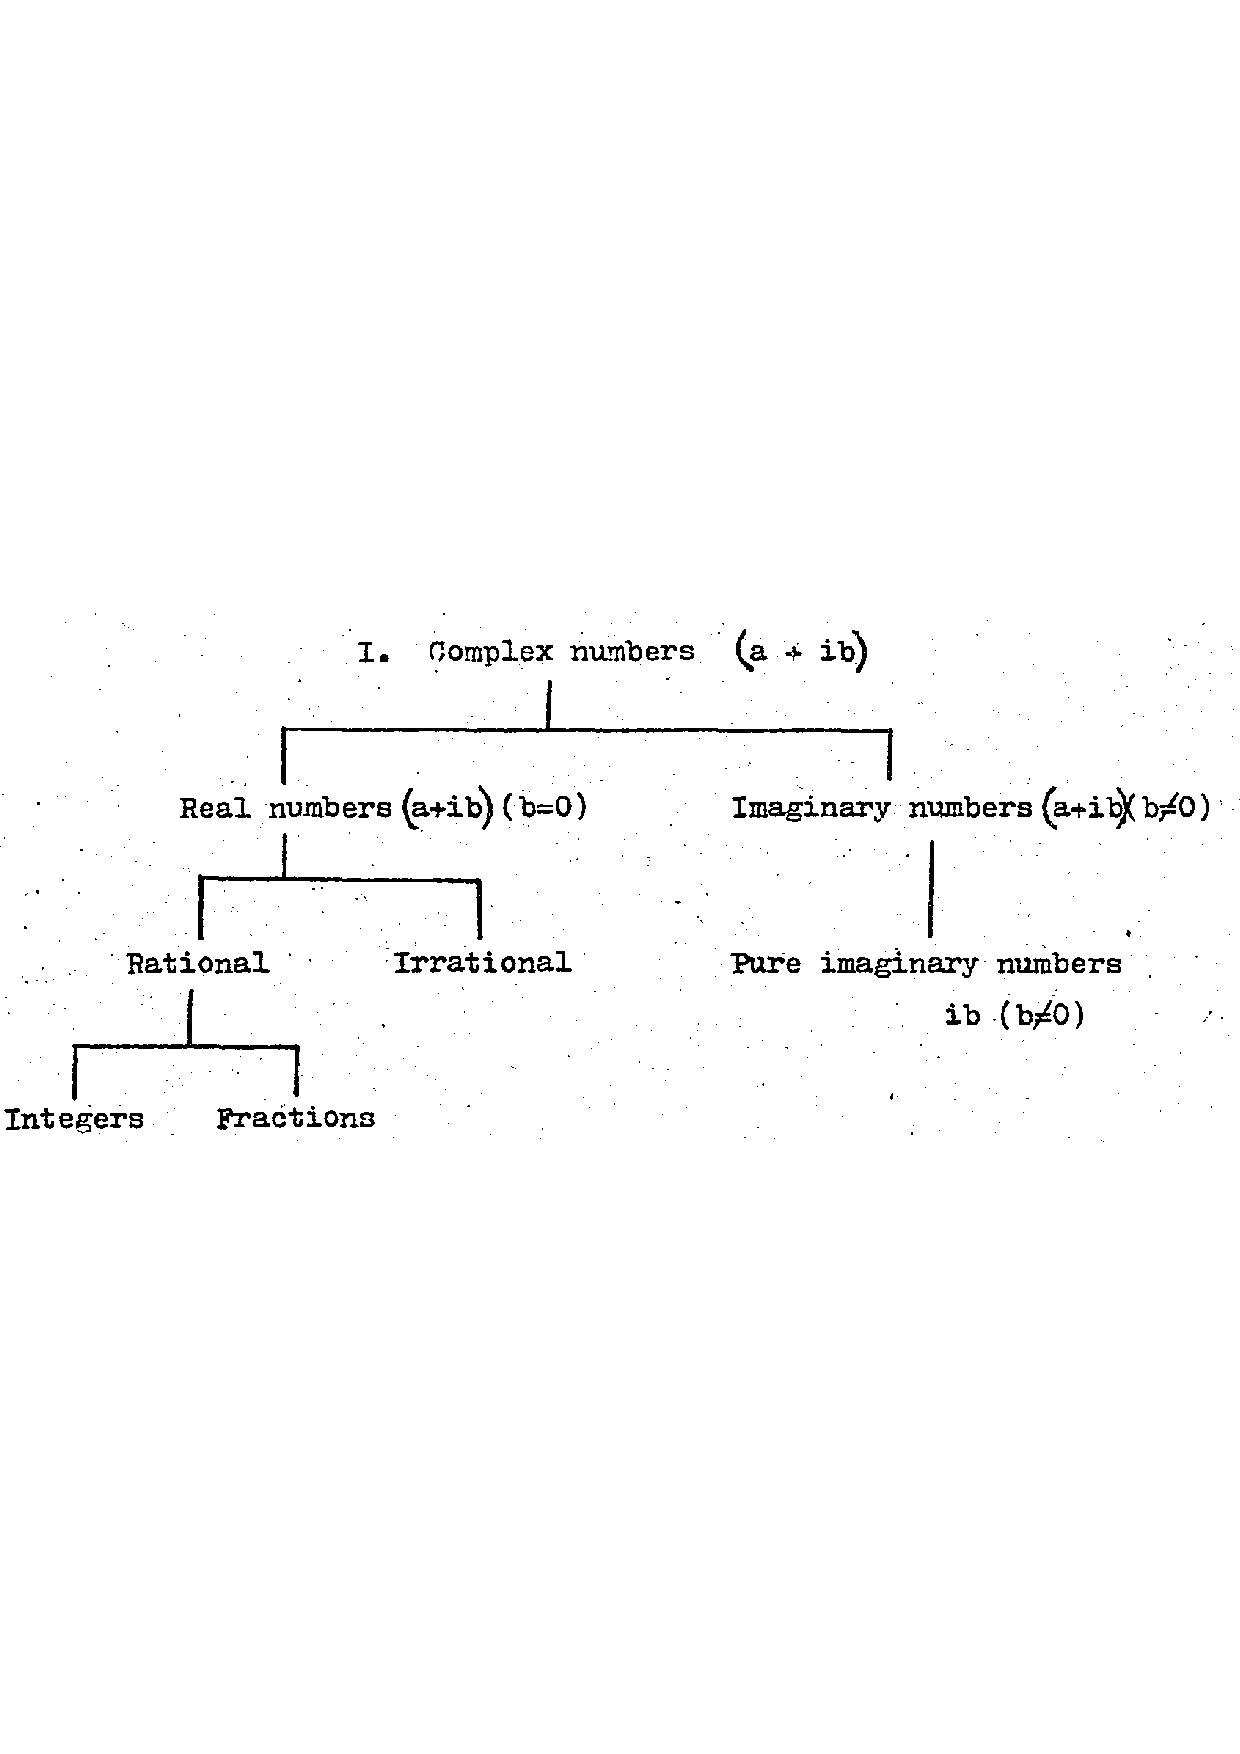
\includegraphics[width=0.9\textwidth]{images/SD-1-1p15A}
%	\caption{Classification of complex numbers}
%	\label{fig:classificationOfComplexNumbersA}
%\end{figure}

%\begin{center}
%\begin{tabular}{cc}
%\end{tabular}
%\end{center}

%\begin{exmp}
%\begin{hSolution}
%\end{hSolution}
%\end{exmp}

%\begin{hEnumerateAlpha}
%\end{hEnumerateAlpha}

%\begin{hEnumerateRoman}
%\end{hEnumerateRoman}

%$
%\begin{bmatrix}
%\end{bmatrix}
%$

%\frac{aaaa}{bbb}
%\frac{a_{n}}{b_{n}}
%\left( aaaa \right)
%\Longrightarrow

%\begin{multicols}{2}
%	bb
%\columnbreak
%	aa
%\end{multicols}
